
%\documentstyle [12pt,psfig] {report}
\documentclass[12pt, openright, psfig]{article}
\usepackage{graphicx}
\usepackage{amsfonts}
\usepackage{verbatim}
\usepackage{subfigure}
%\usepackage{float}
\usepackage{lscape}
%\usepackage{rotating}
\usepackage{setspace}

%\input{cuthesis.sty}
%\begin{comment}
\newenvironment{narrow}[2]{%
%	\begin{list}{}{%
%	\setlength{\topsep}{0pt}%
	\setlength{\leftmargin}{#1}%
	\setlength{\rightmargin}{#2}%
%	\setlength{\listparindent}{\parindent}%
%	\setlength{\itemindent}{\parindent}%
%	\setlength{\parsep}{\parskip}%
%\item[]} {\end{list}
}
%\end{comment}


\newcommand{\LY} {\textrm{L1}}
\newcommand{\LE} {\textrm{L2}}
\newcommand{\LS} {\textrm{L3}}
\newcommand{\LF} {\textrm{L4}}
\newcommand{\LW} {\textrm{L5}}
\newcommand{\PLAUT} {\textsc{Plaut04}}

\newcommand{\LIB}[1] {\textrm{L{#1}}}

\newcommand{\V}[1] {\ensuremath {\textbf V{{#1}}}}
\newcommand{\LYAP}[1] {\ensuremath {\textbf L{{#1}}}}
\newcommand{\W}[1] {\ensuremath {\textbf W{{#1}}}}
\newcommand{\HALO}[1] {\ensuremath {\textbf  H{{#1}}}}
\newcommand{\A}[1] {\ensuremath {\textbf  A{{#1}}}}
\newcommand{\PLAN}[1] {\ensuremath {\textbf  P{{#1}}}}
\newcommand{\LONG}[1] {\ensuremath {\textbf  L{{#1}}}}
\newcommand{\B}[1] {\ensuremath {\textbf  B{{#1}}}}
\newcommand{\D}[1] {\ensuremath {\textbf  D{{#1}}}}
\newcommand{\X}[1] {\ensuremath {\textbf  X{{#1}}}}
\newcommand{\C}[1] {\ensuremath {\textbf  C{{#1}}}}
\newcommand{\SHORT}[1] {\ensuremath {\textbf  S{{#1}}}}
\newcommand{\BP}[2] {\ensuremath {\textsl{#1} {{#2}}}}



% font for the test cases items
\newcommand{\TCF}[1] {\textsl{#1}}
\newcommand{\ETC} {\textit{etc.}}
\newcommand{\PURPOSE} {\subsubsection{Purpose}}
\newcommand{\CMDFMT} {\subsubsection{Format}}
\newcommand{\CMDEXP} {\subsubsection{Examples}}
\newcommand{\DSCP} {\subsubsection{Description}}
\newcommand{\SEEALSO} {\subsubsection{See also}}
\newcommand{\ALIA} {\subsubsection{Aliases}}

\begin{document}

\pagenumbering{roman}
%	\title{How to use AUTO to compute the periodic solutions for the CR3BP}
	\title{\textsc{\PLAUT~User's Guide}}
	\author{Chenghai Zhang, Bart~E.~Oldeman, Eusebius~J.~Doedel}

%	\setcounter{page}{3}
	\date{\today}
	\maketitle
\clearpage

%=========================================================================

%\chapter{User's Guide for \PLAUT} \label{app:userGuide}

``\PLAUT'' is a graphic tool for AUTO data visualization. Here we
explain how to
view AUTO data sets with \PLAUT. An AUTO data set contains a solution file, ``s.foo'', 
a bifurcation file, ``b.foo'', and a diagnostic file, ``d.foo''. Here ``foo'' denotes a user-chosen data set name. 
This user's guide includes the following information:
\begin{enumerate}
    \item A description of the \PLAUT~ window system.
    \item A list of \PLAUT~ configuration options.
    \item An example of using \PLAUT.
\end{enumerate}

\section{Quick start}

\subsection{Starting and stopping \PLAUT }

\subsubsection{Starting}

The starting command for \PLAUT~ is: ``plaut04''. A short Unix command
is also provided as ``@pl''. In the Python CLUI, one can start \PLAUT
~by typing ``plot3()'', ``p3()'', or ``commandPlotter3D()''.
 
This command can have no argument, one argument, or two arguments. 

If no argument is provided, then the system uses the AUTO default data files,  
fort.7, fort.8, and fort.9, as inputs. 

If one argument is given, it must be the name of the data set which we want  
to view. This data set should be in the current directory.

When two arguments are given,
the first is always the path to the data set, and the second is the data set name. 

Note that the AUTO data set name does not mean the full name of an AUTO file. It refers to
the postfix of AUTO data files. For example, if we have the AUTO
data files: ``s.H1'', ``b.H1'', and ``d.H1'', the AUTO data file name is ``H1''.

\subsubsection{Stopping}

One can exit the system by
clicking the cross at the top-right corner of the window or from the ``File'' menu of the system.
\begin{comment}
\begin{figure}[!htmb]
	\captionstyle{center}
\centering
\scalebox{.50}{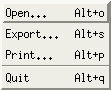
\includegraphics {./include/exit.pdf}}
%\makebox[\textwidth]{\framebox[5cm]{\rule{0pt}{5cm}}}
\caption{Exit the System} \label{fig:exitSys}
\end{figure}
\end{comment}

\subsection{Changing the ``Type''}

Often one will frequently change between the solution diagram and the bifurcation diagram.
The ``Type'' menu helps to complete this change. This menu includes two
items, ``Solution'', and ``Bifurcation''. There is a marker beside the current
diagram. For example, if the current diagram is the solution diagram, 
but we want to change to the bifurcation diagram, 
we can do so by clicking ``Type $\to$ Bifurcation'' to switch to the
bifurcation diagram. 

\begin{figure}[!htmb]
    \begin{minipage}[b]{0.5\textwidth}
        \begin{center}
        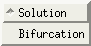
\includegraphics {./include/typeMenu.pdf}
        \caption{The Type Menu} \label{fig:tpyeMenu}
	\end{center}
    \end{minipage}%
    %\hspace{0.0\textwidth}%
    \begin{minipage}[b]{0.5\textwidth}
        \begin{center}
        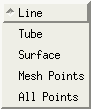
\includegraphics {./include/styleMenuNew.pdf}
        \caption{The Style Menu} \label{fig:styleMenu}
	\end{center}
    \end{minipage}
\end{figure}

\subsection{Changing the ``Style''}

\PLAUT~ provides four ways to draw the graphics, \textit{i.e.}, using 
curves, tubes, points, or as a surface. One can select the style from 
the ``Style'' menu. The ``Style'' menu is shown in Figure \ref{fig:styleMenu}.

\subsection{Coordinate axes} 

Figure \ref{fig:coordMenu} shows the selections of the ``Coord'' menu.
One may use this menu to select to show or not to show 
coordinate axes, and the type of coordinate axes, in the graphics.

\subsection{Options}

The ``Options'' Menu provides functions to add or remove widgets from the graphics.
It also allows to start/stop solution or orbit animation.
The ``normalize data'' normalizes the raw data to [0,1]. 
``Preference'' lets  us set preferences for the GUI (see Figure \ref{fig:optionMenu}). 
\begin{figure}[!htmb]
	\centering
    \begin{minipage}[b]{0.5\textwidth}
        \centering
        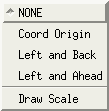
\includegraphics {./include/drawCoordMenu.pdf}
        \caption{The Draw-Coordinate-Axes Menu} \label{fig:coordMenu}
    \end{minipage}%
    %\hspace{0.2\textwidth}%
    \begin{minipage}[b]{0.5\textwidth}
        \centering
        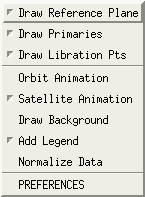
\includegraphics {./include/optionMenu.pdf}
    	\caption{The Options Menu} \label{fig:optionMenu}
    \end{minipage}
\end{figure}

\subsection{CR3BP animation}

The ``Center'' Menu allows to animate the motion of the three bodies in different
coordinate systems. We can animate the motion in a large-primary-centered inertial 
coordinate system, or in a small-primary-centered inertial system, or in the bary-centered
inertial system. Figure \ref{fig:centerMenu} displays the layout of the ``Center'' menu. 

\begin{figure}[!htmb]
\centering
    \begin{minipage}[b]{0.5\textwidth}
        \centering
        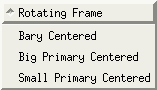
\includegraphics {./include/centerMenu.pdf}
        \caption{The Center Menu} \label{fig:centerMenu}
    \end{minipage}%
    %\hspace{0.2\textwidth}%
    \begin{minipage}[b]{0.5\textwidth}
        \centering
        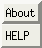
\includegraphics {./include/helpMenu.pdf}
        \caption{The Help Menu} \label{fig:helpMenu}
    \end{minipage}
\end{figure}


\subsection{Help}

The ``Help'' menu provides an on-line help on how to use \PLAUT.

\subsection{Picking a point in the diagram}

The picking operation is useful when we want to know data corresponding to a certain
point in the diagram. In order to execute a picking operation, we should follow these steps.
\begin{itemize}
	\item Click the arrow icon to change the mouse to picking state. 
    \item Move the mouse to the point of interest.
	\item Click the left button of the mouse to pick the point.
\end{itemize}

Once a point has been picked, a new window is popped up. In this new window, the Floquet
multipliers of the point are shown in an x-y plane.  
Black crosses in the diagram indicate the Floquet Multipliers.
The solution, and the values of the corresponding Floquet Multipliers, are given in the lower part of the
window. A unit circle is drawn in the diagram.
Figure \ref{fig:flq} is an example of the picking operation.
From this diagram, we can see that two Floquet Multipliers
are outside the unit circle, two are on the unit circle, and the other two are inside the unit circle.

\begin{figure}[!htmb]
\centering
\scalebox{.60}{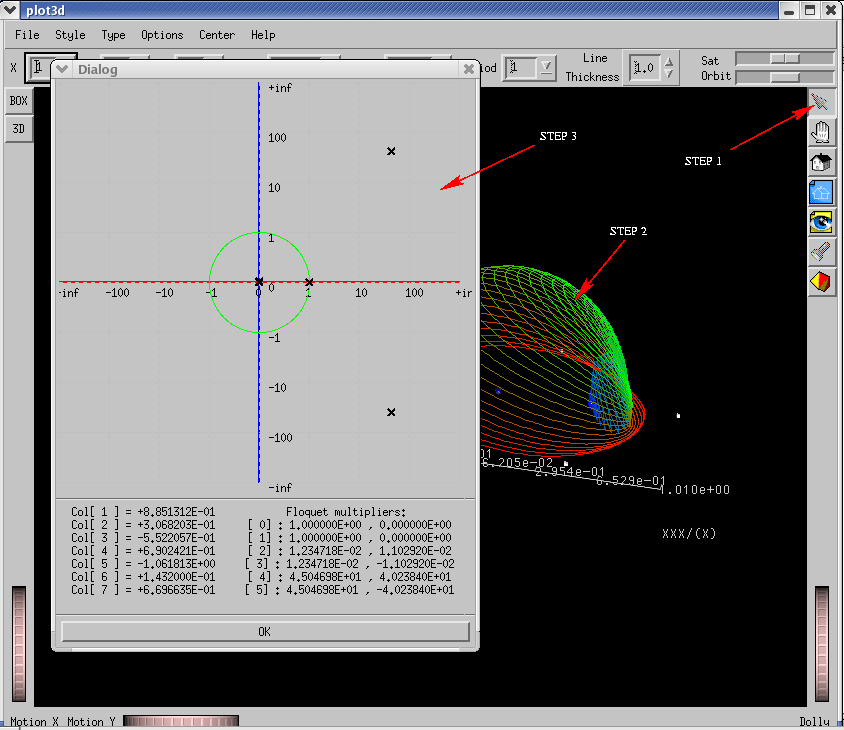
\includegraphics {./include/floquet.pdf}}
%\makebox[\textwidth]{\framebox[5cm]{\rule{0pt}{5cm}}}
\caption{Picking a point }
\label{fig:flq}
\end{figure}

\subsection{Choosing the variables}

\begin{figure}[!htmb]
\centering
\scalebox{.60}{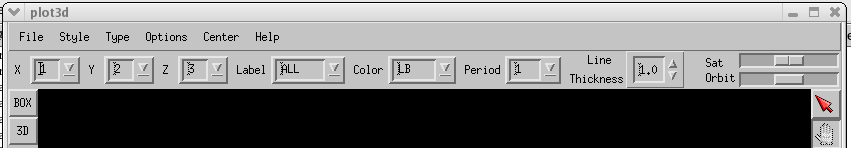
\includegraphics {./include/menubar.pdf}}
%\makebox[\textwidth]{\framebox[5cm]{\rule{0pt}{5cm}}}
\caption{Menu-bar layout}
\label{fig:mnbar}
\end{figure}

AUTO can generate large amounts of data. The CR3BP, for example, has 6 variables, \textit{i.e.}, $x,y,
z, x', y', z'$, and time. One can choose to draw any combination of these variables in 2  
or 3 dimensions using \PLAUT. On the list bar,  
we can see three {dropdown lists} with label ``X'', ``Y'', and ``Z'' (See Figure~\ref{fig:mnbar}).
Each of these three lists has the exact number of choices, namely, the number of variables of the system plus one.
In our case, these lists have 7 choices, which are represented by the integers 0 to 6. 
0 represents time. 1 to 6 stand for $x, y, z, x', y'$, and $z'$, respectively. 
``1'' is selected for ``X'', which indicates that $x$ is drawn on the X-axis. 
``2'' is selected for ``Y'',  which indicates that $y$ is represented on the Y-axis. 
``3'' is selected for ``Z'',  which indicates that $z$ is represented on the Z-axis. 

\begin{figure}[!htmb]
\centering
\scalebox{.50}{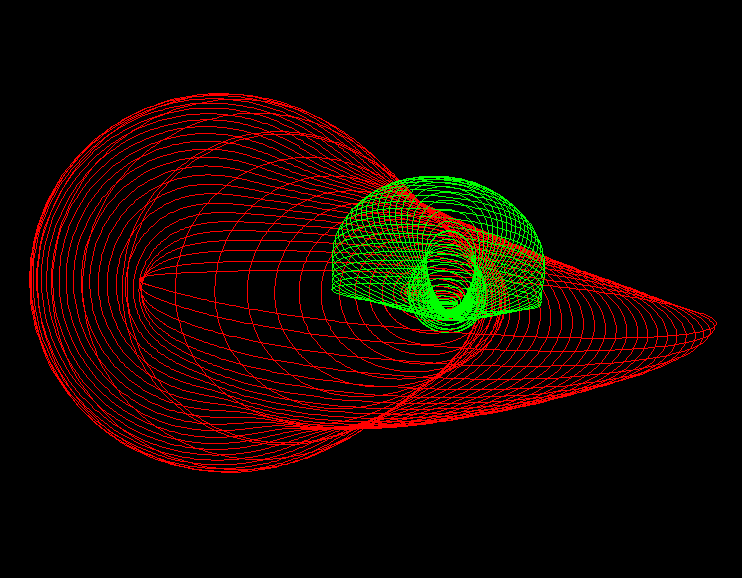
\includegraphics {./include/2component.pdf}}
%\makebox[\textwidth]{\framebox[5cm]{\rule{0pt}{5cm}}}
\caption{Displaying multiple components}
\label{fig:twoPairs}
\end{figure}

We can also show multiple combinations at the same time. For example, if we want 
to show x-y-z and x'-y'-z' in the same diagram, we can input $1,4$ in the ``X'' \textrm{dropdown list} to 
select $x$ and $x'$ being drawn on the X-axis, input $2,5$ in the ``Y'' list to show $y$ and $y'$ on the Y-axis,
and input $3,6$ in the ``Z'' \textrm{dropdown list} to draw $z$ and $z'$ on the Z-Axis. Note that after finishing 
the input in the \textrm{dropdown list} box, we must type ``ENTER'' for  
the input to be accepted by the system. Figure \ref{fig:twoPairs} shows the results of the above
choices. The combination is flexible. For example, if X is $1$, Y is $3, 5$, and Z is $4, 5, 6$, 
the system will automatically reorganize them to $1-3-4$, $1-5-5$, $1-3-6$ and show the results.
If X is $1, 5$,  Y is $2$, and Z is $3, 4$, the system reorganizes them to $1-2-3$, $5-2-4$.

Different components are drawn with different colors from blue to red. 

The default values can be set in the resource file. If no resource file exists, then the system
will use ``1'' for X-axis, ``2'' for Y-axis, and ``3''for Z-axis for both the solution and the bifurcation
diagrams.

\subsection{Choosing labels}

From the Label list, we can choose the label of the solution to be drawn. If ``ALL'' is chosen, all 
solutions are shown in the diagram. If ``NONE'' is chosen, none of the solutions is shown.
``HALF'' shows the solutions with odd labels and special solutions only. ``SPEC'' lets the system
show the special solutions only.
We can also show selected solutions by inputting their labels in the list
box separated by commas. 
For example, typing 1, 10, 15, 20 will lead the system to show only the solutions with label 1, 10, 15 and 20. 

We can set the default value for this list in the \PLAUT~resource file.

\subsection{Coloring}

Many coloring methods are provided. They can be classified into three groups. The first group
is coloring by variables. 
This group provides as many choices as the number of variables of a problem plus
1 for the time. 
The second group is coloring by parameters. These parameters are defined by the AUTO user. 
in the AUTO constants file. 
There are as many choices as the number of parameters defined in the AUTO constants file.
The third group includes ``TYPE'', type of solution, 
``PONT'', point number, 
``BRAN'', the branch to which the solution belongs, 
and ``LABL'', label of the solution. 
Different coloring methods cannot be used at the same time.
Figure \ref{fig:clrMethod} shows the difference between coloring by type and coloring by label. 
From Figure \ref{fig:clrMethod}(a), we can see that there is only one
branching orbit in this family, which is shown in cyan. 
In Figure~\ref{fig:clrMethod}(b), the start solution is colored in blue, and the last solution is colored in red. 
When using time to color the diagram, 0 is set to blue, while 1 is set to red. 
\begin{figure}[!htmb]
    \subfigure[Coloring by ``Type'']{
    \label{fig:clrType}
    \begin{minipage}[b]{0.32\textwidth}
        \centering
        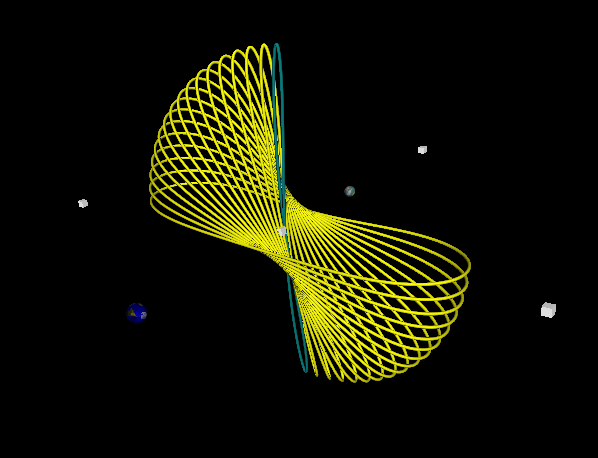
\includegraphics[width=5.0cm, height=5.0cm] {./include/clrTyMu0.pdf}
    \end{minipage}}%
    \subfigure[Coloring by ``Label'']{
    \label{fig:clrLabel}
    \begin{minipage}[b]{0.32\textwidth}
        \centering
        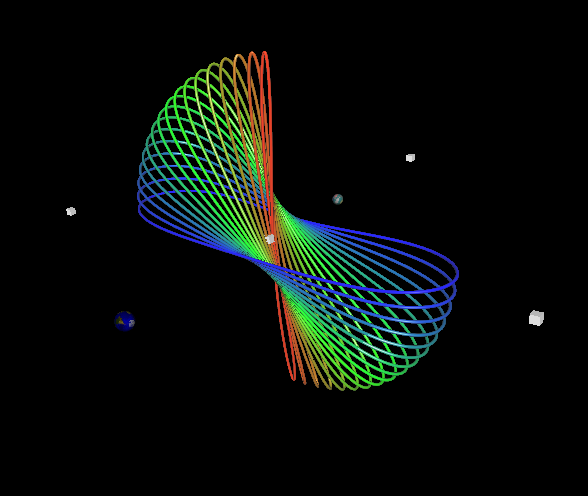
\includegraphics[width=5.0cm, height=5.0cm]{./include/clrLBMu0.pdf}
    \end{minipage}}%
    \subfigure[Coloring by ``Time'']{
    \label{fig:clrTime}
    \begin{minipage}[b]{0.32\textwidth}
        \centering
        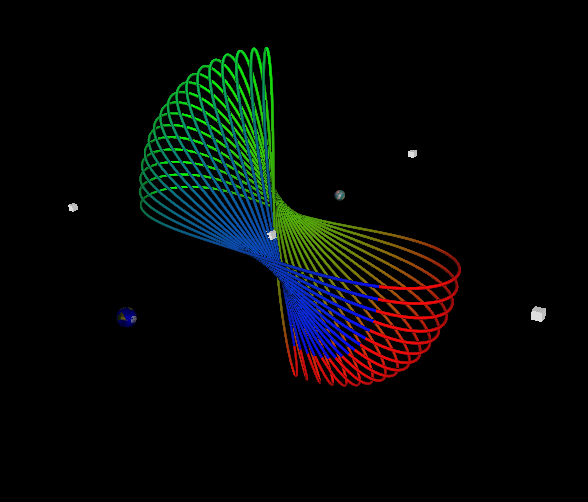
\includegraphics[width=5.0cm, height=5.0cm]{./include/clrTimeMu0.pdf}
    \end{minipage}}
    \caption{Coloring} \label{fig:clrMethod}
\end{figure}

We can set the default value in the \PLAUT~resource file.

\subsection{Number of periods to be animated}

Generally only one period is animated when we animate the solution in the inertial frame.
However, the SpinBox allows us to change the default value. 
 This is a specially designed function for the CR3BP. 
It is useful when  we animate the motion in the three bodies in the inertial frame.

\subsection{Changing the line/tube thickness}

The ``Line Thickness'' spinbox allows us to increase or decrease the line/tube thickness
in the diagram.  The \PLAUT~ resource file also provides a way to change the default values of the
line/tube thickness.

\subsection{Changing the animation speed}

The ``Sat'' and ``Orbit'' scale bar allow us to change the animation speed. 
Their Maximum and Minimum value can be set in the resource file.

\subsection{Changing the background picture}

A user can set the background with his favorite picture. 
To do this, a user should copy the picture to the directory ``\$AUTO\_DIR/plaut04/widgets'', 
and then change the name of the file to ``background.rgb''.

\section{Setting up the resource file}

The \PLAUT~resource file sets default values for 
almost all controls of \PLAUT. 
%Generally when we solve a problem, we want
%to put the solutions in the same directory. 
%For the same problem, what a user is interested in is almost the same.  
\PLAUT~allows us to write our own resources files and put them in the same directory as the AUTO data files. 
\PLAUT~first looks for the resource file in the current directory.
If it cannot find a resource file there, then it will try to use the one installed
in the AUTO root directory. If both these searches fail, then the internal
default values will be used.

In order to write a usable resource file, one should follow the following rules:
\begin{enumerate}
\item Comment lines start with ``\#''. Comments may take as many lines as desired.
\item Between the ``variable name'' and the default value, we must use 
``='' to tell the system that the left side is the ``variable name'', and
the right side is its corresponding default value.
\item If a ``variable'' has aggregate values, a comma ``,'' must be used between
two values.
\item The line type is set using 4-digit hexadecimals, starting with ``0x''. Its values can 
range from $0$ (invisible) to ``0xffff'' (solid). The system default is ``0xffff'' for stable
solutions, and ``0x3333'' for unstable ones. 
The line pattern is determined by the number of $1$s and $0$s when the hexadecimal
is converted to a $16$-bit binary. A ``$1$'' indicates that the drawing occurs, and ``$0$'' that 
it does not, on a pixel by pixel basis. For example, the pattern ``0xAAAA'', 
in binary is $0000100010001000$, and \PLAUT~interprets this as drawing 
3 bits off, 1 bit on, 3 bits off, 1 bit on, 3 bits off, 1 bit on and finally 4 bits off.
The pattern is read backward because the low order bits are used first.
\item Some variables can only be set to ``Yes'' or ``No''. They cannot be assigned other values.
\item No ``variable name'' should be  modified.
\end{enumerate}

It is strongly recommended that the default resource file is used as a template
when writing a custom resource file. 

Below is a copy of the default resource file. 
{\footnotesize
\begin{verbatim}
#version 0.0

# Line colors are represented by RGB values from 0 to 1.0.
# DEFAULT color is also used when animationLabel == 0, i.e.,
# when showing all solutions and animating the solution change.
# Point Type    RED  GREEN  BLUE PATTERN
DEFAULT       = 1.0,  1.0,  1.0, 0xffff
BP ALG        = 1.0,  0.0,  0.0, 0xffff
LP ALG        = 0.0,  1.0,  0.0, 0xffff
HB            = 0.0,  0.0,  1.0, 0xffff
UZ4           = 1.0,  1.0,  0.0, 0xffff
UZ-4          = 0.5,  0.5,  0.0, 0xffff
LP DIF        = 0.0,  0.0,  0.5, 0xffff
BP DIF        = 0.0,  0.5,  0.5, 0xffff
PD            = 1.0,  0.0,  1.0, 0xffff
TR            = 0.0,  1.0,  1.0, 0xffff
EP            = 0.3,  0.0,  0.3, 0xffff
MX            = 0.6,  0.0,  0.6, 0xffff
OTHERS        = 1.0,  1.0,  1.0, 0xffff

# Initialize the line pattern for showing stability:
UNSTABLE LINE PATTERN = 0xffff 
STABLE LINE PATTERN   = 0xffff

# Initialize the default options:
Draw Reference Plane  = No
Draw Reference Sphere = No
Orbit Animation       = No
Satellite Animation   = No 
Draw Primaries        = No 
Draw Libration Points = No 
Normalize Data        = No
Draw Labels           = No
Show Label Numbers    = No
Draw Background       = No
Draw Legend           = No

# Initialize the default coordinate axes:
#  0 --- None,
#  1 --- at origin
#  2 --- at left and behind
#  3 --- at left and ahead
#  4 --- always at origin
Coordinate Type = 3

# Draw Scale on the Aexs
Draw Scale = Yes 

#  Initialize the default graph type:
#  0 --- Solution (fort.8)
#  1 --- Bifurcation (fort.7)
Graph Type    = 0

# Initialize the default graph style:
#  0 --- LINES,
#  1 --- TUBES,
#  2 --- SURFACE
Graph Style  =  0

# Set the window width and height:
Window Width        = 1000
Window Height       = 1000 

# Set X, Y, Z axes for the solution diagram:
# 0 is Time for X,Y,Z.
X Axis Solution             = 1
Y Axis Solution             = 2
Z Axis Solution             = 3

# Set X, Y, Z axes for the bifurcation diagram:
X Axis Bifurcation          = 4
Y Axis Bifurcation          = 5
Z Axis Bifurcation          = 6

#Labeled solutions:
Labels              = 0

# Set coloring method:
# -6 --- STABILITY
# -5 --- POINT
# -4 --- BRANCH
# -3 --- TYPE 
# -2 --- LABEL 
# -1 --- COMPONENT 
# Otherwise, according to the data in the ith column of the solution file.
# It can only be set to an integer value.
#Coloring Method           = -3
# For the solution diagram:
Coloring Method Solution  = -3
# For the bifurcation diagram:
Coloring Method Bifurcation = -3
Number of Period Animated = 1

# Line Width Scaler adjusts the thickness of curves:
Line Width Scaler         = 1.0

# The AniLine Thickness Scaler sets the thickness of animated solution curves:
AniLine Thickness Scaler  = 3.0

# Background color:
Background Color  = 0.0,  0.0,   0.0

# Background transparency:
Background Transparency = 0.0 

# Set the radius of the spheres used for labels:
# The normal size is 1.0.
# For smaller radius, use 0.xxx
# For bigger radius, use  X.XXX
Label Sphere Radius       =  1.0

# Disk Rotation
Disk Rotation = 1.0, 0.0, 0.0, 1.570796

# Disk Position
Disk Position = 0.0, 0.0, 0.0

# Disk Radius
Disk Radius = 1.0

# Disk Height
Disk Height = 0.001

# Disk Transparency [0, 1]
Disk Transparency = 0.7 
 
# Read Disk From File
Disk From File = No 
 
# Sphere Position
Sphere Position = 0.0, 0.0, 0.0

# Sphere Radius
Sphere Radius = 1.0

# Sphere Transparency [0, 1]
Sphere Transparency = 0.7

# Read Sphere From File
Sphere From File = No

# Axes color:
X Axis Color    = 1.0,  0.0,   0.0
Y Axis Color    = 0.0,  1.0,   0.0
Z Axis Color    = 0.0,  0.0,   1.0

# Color of the satellite, large primary, and small primary in animation:
satellite Color             = 1.0,  0.0,   0.0
large primary Color         = 0.0,  1.0,   0.0
large primary tail Color    = 0.0,  1.0,   1.0
small primary Color         = 0.0,  0.0,   1.0
small primary tail Color    = 0.5,  0.5,   0.0

# Surface color:
Surface Color         =  0.0,  1.0,  0.0

# Stable solution color:
Stable Solution Color = 0.0, 0.0, 1.0

# Stable solution color:
Unstable Solution Color = 1.0, 0.0, 0.0

# Set the radius of the satellite, large primary, and small primary:
# The normal size is 1.0.
# For smaller radius, use 0.xxx
# For bigger radius, use  X.XXX
Satellite Radius        = 1.0
Large Primary Radius    = 1.0
Small Primary Radius    = 1.0
Libration Point Size    = 1.0

# Set the initial, maximum and minimum satellite animation speed:
Sat Animation Speed = 100
Sat Max Animation Speed = 100
Sat Min Animation Speed = 0

# Set the initial, maximum and minimum orbit-change animation speed:
Orbit Animation Speed = 50
Orbit Max Animation Speed = 100
Orbit Min Animation Speed = 0

# Set the active AUTO parameter indices:
parameter ID = 10

# Choose 3D or 2D graph:
#3D  = Yes 

# Choose 3D or 2D graph for the bifurcation diagram:
3DBif = Yes

# Choose 3D or 2D graph for the solution diagram:
3DSol = Yes

\end{verbatim}
}

\section{Example}

In this example, we want to view a CR3BP data set.
We want the diagram to show the ``$x$'' component on the X-axis, ``$y$'' component on the Y-axis, and ``$z$'' component on the Z-axis
for the solution diagram. 
%and column 4 of the AUTO b file as the X-axis, column 5
%on the Y-axis, and column 6 on the Z-axis, for the bifurcation diagram. 
In the CR3BP, we use the parameters ``1 2 3 10 21 22 23'' in the AUTO  
calculations, and we also want to be able to use these to color the diagram, so we set the ``parameter indices''.  

Other preferences include
\begin{itemize}
\item The diagram is drawn using Tubes.
\item Coordinate axes are not drawn.
\item No animation.
\item Reference plane, libration points, and primaries are drawn.
\item All labels are shown.
\item Data is not normalized. 
\end{itemize}

The settings are the settings in the resource file are then as follows:
{\footnotesize
\begin{verbatim}
#  Initialize the default options
Draw Reference Plane  = Yes
Orbit Animation       = No
Satellite Animation   = No 
Draw Primaries        = Yes
Draw Libration Points = Yes
Normalize Data        = No
Draw Background       = No

#  Initialize the default graph type
#  0 --- Solution(fort.8)  1 --- Bifurcation(fort.7)
Graph Type    = 0

# initialize the default graph style
#  0 --- LINES,  1 --- TUBES, 2 ---- SURFACE  3--- nurbs curve
graph Style  =  1

# set X, Y, Z, and Label
# 0 is Time for X,Y,Z. 0 is "All" for Label

Solution X Axis              = 1
Solution Y Axis              = 2
Solution Z Axis              = 3

Labels                       = 0

#set the parameter indices 
parameter ID = 1,  2,  3, 10,  15, 21, 22,  23
\end{verbatim}
}

Based on the above settings, 
the solution diagram for the CR3BP family \L{1} for $\mu=0.01215$ appears in Figure \ref{fig:AppEx1}.

\begin{comment}
\begin{figure}[!htmb]
	\centering
	%\includegraphics[width=10cm] {./include/ex1Mu0.01215V1.pdf}
	%\includegraphics[width=10cm] {./include/emV4Surface.pdf}
	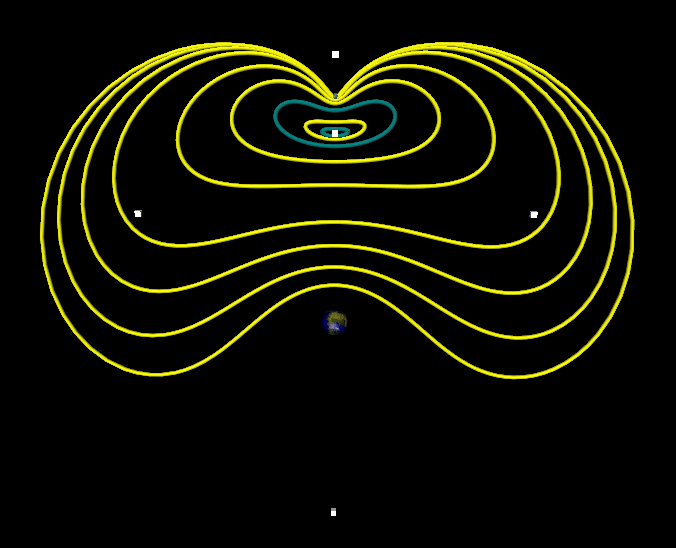
\includegraphics[width=10cm] {./include/emL1Sol.pdf}
%\makebox[\textwidth]{\framebox[5cm]{\rule{0pt}{5cm}}}
	\caption{Example}
\label{fig:AppEx1}
\end{figure}
\end{comment}

\begin{figure}[!htmb]
        \centering
		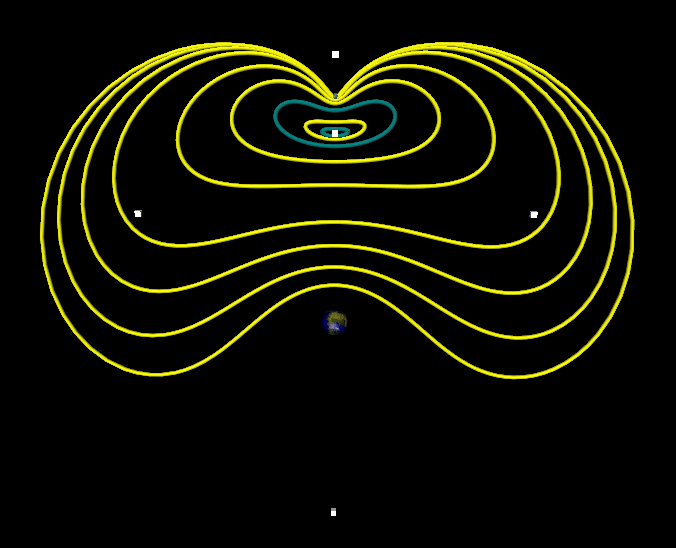
\includegraphics[width=10cm, height=10cm] {./include/emL1Sol.pdf}
        \caption{Example} \label{fig:AppEx1}
\end{figure}



\end{document}
